% questions.tex —— 1987 年·广东卷·理工农医类 · 题目内容片段（无答案）
% 由 tools/generate_projects.py 依来源总账自 1987/1987_数学真题_广东理_试题.md 生成，勿手改（改源 MD 后重跑）


\gkpart{试题}

\begin{gktip}
\textbf{来源说明}：本题面依据固定源 PDF《1987 年广东省高考数学（理工农医类）试题与解答》逐题转录。固定源共 10 页，题面为 PDF 第 1—5 页，答案与解答为第 6—10 页；原卷版面没有连续印刷页码。

\textbf{图形说明}：第二卷第二题的三棱台图依据固定源图形关系重绘为 TikZ 矢量图。第 1 题第 17 小题和第 22 小题分别存在题面—答案冲突与选项图形缺失，均照录并列入问题总账。固定源文本层中的私有字形乘号按视觉读取为乘法点号，并在问题台账中保留说明。
\end{gktip}

\begin{question}
\gkti{1}

第一卷共 25 个选择题，每题只有一个结论正确。

\Needspace{5\baselineskip}
（1） 函数

\nopagebreak[4]
\[
y=\sqrt{2x-x^2}
\]

的定义域是\mbox{（　　）}

（A）$(-\infty,0)$　　（B）$(0,2)$　　（C）$[0,2]$　　（D）$[-2,0]$

\Needspace{5\baselineskip}
（2） 方程

\nopagebreak[4]
\[
2\cdot4^x-5\cdot2^x+2=0
\]

的解集是\mbox{（　　）}

（A）$\{1\}$　　（B）$\{\frac12,1\}$　　（C）$\{-1,\frac12\}$　　（D）$\{-1,1\}$

\Needspace{5\baselineskip}
（3） 使函数

\nopagebreak[4]
\[
y=\cos2x
\]

取最小值的所有 $x$ 的集合是\mbox{（　　）}

（A）$\{x\mid x=\pi+k\pi,\ k\in\mathbb Z\}$

（B）$\{x\mid x=\frac\pi2+k\pi,\ k\in\mathbb Z\}$

（C）$\{x\mid x=\pi+2k\pi,\ k\in\mathbb Z\}$

（D）$\{x\mid x=\frac\pi2+2k\pi,\ k\in\mathbb Z\}$

（4） 如果圆锥的高和底面直径都等于 $a$，则该圆锥的体积为\mbox{（　　）}

（A）$\frac\pi4a^3$　　（B）$\frac\pi6a^3$　　（C）$\frac\pi{12}a^3$　　（D）$\frac\pi3a^3$

\Needspace{5\baselineskip}
（5） 在圆

\nopagebreak[4]
\[
x^2+y^2=4
\]

\Needspace{5\baselineskip}
上，与直线

\nopagebreak[4]
\[
4x+3y-12=0
\]

距离最小的点的坐标是\mbox{（　　）}

（A）$\left(\frac85,\frac65\right)$　　（B）$\left(\frac85,-\frac65\right)$

（C）$\left(-\frac85,\frac65\right)$　　（D）$\left(-\frac85,-\frac65\right)$

\Needspace{5\baselineskip}
（6） 若复数

\nopagebreak[4]
\[
z=(a+i)^2
\]

的辐角是 $\frac32\pi$，则实数 $a$ 的值为\mbox{（　　）}

（A）$1$　　（B）$-1$　　（C）$-\sqrt2$　　（D）$\sqrt3$

\Needspace{5\baselineskip}
（7） 不等式

\nopagebreak[4]
\[
\frac{3x-1}{2-x}\geq1
\]

的解集是\mbox{（　　）}

（A）$\left\{x\mid\frac34\leq x\leq2\right\}$

（B）$\left\{x\mid\frac34\leq x<2\right\}$

（C）$\{x\mid x>2\ \mathrm{or}\ x\leq\frac34\}$

（D）$\{x\mid x<2\}$

（8） 若 $\operatorname{ctg}\frac\theta2=3$，则 $\cos\theta$ 的值是\mbox{（　　）}

（A）$\frac35$　　（B）$-\frac35$　　（C）$-\frac45$　　（D）$\frac45$

\Needspace{5\baselineskip}
（9） 在闭区间 $[-\pi,\pi]$ 上，方程

\nopagebreak[4]
\[
\frac1{|\sin x|}=\sin x-\cos x
\]

的不同实根个数是\mbox{（　　）}

（A）2　　（B）3　　（C）4　　（D）5

（10） 用 $0,1,2,3$ 这四个数字，组成个位数不是 1 的没有重复数字的四位数，共有\mbox{（　　）}

（A）16 个　　（B）14 个　　（C）12 个　　（D）10 个

\Needspace{5\baselineskip}
（11） 设

\nopagebreak[4]
\[
f(x)=\frac{2x+1}{4x+3}\qquad(x\in R,\ x\ne-\frac34),
\]

\Needspace{5\baselineskip}
则

\nopagebreak[4]
\[
f^{-1}(2)=
\]

（A）$-\frac56$　　（B）$\frac5{11}$　　（C）$\frac25$　　（D）$-\frac25$

\Needspace{5\baselineskip}
（12） 圆锥曲线

\nopagebreak[4]
\[
y^2-4y+4x=0
\]

的准线方程是\mbox{（　　）}

（A）$x=0$　　（B）$x=-1$　　（C）$x=1$　　（D）$x=2$

\Needspace{5\baselineskip}
（13） 设常数 $a>0$，椭圆

\nopagebreak[4]
\[
x^2-2ax+a^2y^2=0
\]

的长轴是短轴的 2 倍，则 $a=$\mbox{（　　）}

（A）$2$ 或 $\frac12$　　（B）$2$　　（C）$\frac12$　　（D）$\sqrt2$

（14） 设双曲线的半焦距为 $c$，两条准线距离为 $d$，且 $c=d$，则这双曲线的离心率 $e=$\mbox{（　　）}

（A）$\sqrt3$　　（B）$\sqrt2$　　（C）$2$　　（D）$3$

\Needspace{5\baselineskip}
（15） 设实数 $\theta\in\left(\frac\pi2,\frac34\pi\right)$，那么方程

\nopagebreak[4]
\[
\frac{x^2}{\csc\theta-2}+\frac{y^2}{2-\sec\theta}=1
\]

所表示的曲线是\mbox{（　　）}

（A）焦点在 $y$ 轴上的椭圆　　（B）焦点在 $x$ 轴上的椭圆

（C）焦点在 $y$ 轴上的双曲线　　（D）焦点在 $x$ 轴上的双曲线

（16） 若正三棱锥的一个侧面的面积与底面的面积的比等于 $\frac23$，则这个三棱锥的侧面和底面所成的二面角是\mbox{（　　）}

（A）$\arccos\frac34$　　（B）$\arcsin\frac34$　　（C）$30^\circ$　　（D）$60^\circ$

（17） 设 $\alpha,\beta$ 是不重合的两个平面，$l,m$ 是不重合的两条直线，那么 $\alpha\parallel\beta$ 的一个充分条件是\mbox{（　　）}

（A）$l\subset\alpha,\ m\subset\alpha$，且 $l\parallel\beta,\ m\parallel\beta$

（B）$l\subset\alpha,\ m\subset\beta$，且 $l\parallel m$

（C）$l\perp\alpha,\ m\parallel\beta$，且 $l\parallel m$

（D）$l\parallel\alpha,\ m\parallel\beta$，且 $l\parallel m$

（18） 函数 $y=-\operatorname{ctg}x$（$x\in(0,\pi)$）的反函数可以写成\mbox{（　　）}

（A）$y=\frac\pi2-\arctan x$　　（B）$y=\frac\pi2+\arctan x$

（C）$y=\pi-\arctan x$　　（D）$y=\pi+\arctan x$

\Needspace{5\baselineskip}
（19） 设

\nopagebreak[4]
\[
(1+x)^3+(1+x)^4+\cdots+(1+x)^{50}
=a_0+a_1x+a_2x^2+a_3x^3+\cdots+a_{50}x^{50},
\]

则 $a_3=$\mbox{（　　）}

（A）$\binom{51}{3}$　　（B）$\binom{51}{4}$　　（C）$2\binom{50}{3}$　　（D）$\binom{50}{4}$

（20） 如果实数 $a,b,c$ 不全为负数，那么\mbox{（　　）}

（A）实数 $a,b,c$ 中，至少有一个正数

（B）实数 $a,b,c$ 中，既有正数又有负数

（C）实数 $a,b,c$ 的乘积不为负数

（D）实数 $a,b,c$ 中，至多有两个负数

（21） 平行六面体成为直平行六面体的一个充分必要条件是\mbox{（　　）}

（A）它有两个矩形的侧面

（B）它的一条侧棱垂直于底面的两条边

（C）它有两条侧棱都垂直于底面的一条边

（D）它有两个侧面都垂直于底面

（22） 若动点 $P$ 的横坐标 $x$ 和纵坐标 $y$，使得 $\lg y,\lg|x|,\lg\left(\frac{y-x}{2}\right)$ 成等差数列，则动点 $P$ 的轨迹图形是\mbox{（　　）}

\begin{gktip}
\textbf{固定源缺失}：本题题干后的 A—D 图形选项在固定源 PDF 中整段缺失，故不补画、也不擅自转录选项。按可见题干独立推导，定义域需满足 $y>0$、$x\ne0$、$y-x>0$。
\end{gktip}

\Needspace{5\baselineskip}
（23） 若函数

\nopagebreak[4]
\[
f(x)=\sin\left(\frac43x+\frac52\pi\right)\quad(x\in R),
\qquad
g(x)=\sin(\arccos x)\quad(x\in[-1,1]),
\]

则\mbox{（　　）}

（A）$f(x)$ 是偶函数而 $g(x)$ 是奇函数

（B）$f(x)$ 是奇函数而 $g(x)$ 是偶函数

（C）$f(x)$ 和 $g(x)$ 都是奇函数

（D）$f(x)$ 和 $g(x)$ 都是偶函数

（24） 在直角坐标系中，$\triangle ABC$ 的三个顶点是 $A(0,3),B(3,3),C(2,0)$，若直线 $x=a$ 将 $\triangle ABC$ 分割成面积相等的两部分，则实数 $a$ 的值是\mbox{（　　）}

（A）$\sqrt3$　　（B）$1+\frac{\sqrt2}{2}$　　（C）$1+\frac{\sqrt3}{3}$　　（D）$2-\frac{\sqrt2}{2}$

\Needspace{5\baselineskip}
（25） 若实数 $x,y$ 满足

\nopagebreak[4]
\[
x^2+y^2-2x+4y=0,
\]

则 $x-2y$ 的最大值是\mbox{（　　）}

（A）$\sqrt5$　　（B）$10$　　（C）$9$　　（D）$5+2\sqrt5$

\end{question}
\begin{question}
\gkti{2}

第二卷第一题（本题满分 15 分）共有五个填空小题，每小题 3 分。

\Needspace{5\baselineskip}
（1） 计算下式：

\nopagebreak[4]
\[
\log_2\sqrt2+\log_9 27
\]

的值是 $\underline{\hspace{3em}}$。

\Needspace{5\baselineskip}
（2） 若圆的极坐标方程为

\nopagebreak[4]
\[
\rho=6\cos\theta,
\]

则这个圆的半径是 $\underline{\hspace{3em}}$。

（3） 命题“三个正数 $a,b,c$ 的几何平均数不大于这三个数的算术平均数”用数学符号表示，可写成“如果 $\underline{\hspace{5em}}$，那么 $\underline{\hspace{7em}}$。”

（4） 已知椭圆的两个焦点是 $F_1(0,-1)$ 和 $F_2(0,3)$，并且点 $A(2,1)$ 在该椭圆上，那么，这个椭圆的标准方程是 $\underline{\hspace{7em}}$。

\Needspace{5\baselineskip}
（5） 计算极限：

\nopagebreak[4]
\[
\lim_{n\to\infty}\frac{2^{n-1}-3^n}{2^n+3^{n-1}}
\]

的值是 $\underline{\hspace{3em}}$。

\Needspace{0.4\textheight}
\end{question}
\begin{question}
\gkti{3}

\Needspace{5\baselineskip}
第二卷第二题（本题满分 12 分）。在三棱台

\nopagebreak[4]
\[
A_1B_1C_1-ABC
\]

\Needspace{5\baselineskip}
中，侧棱 $B_1B\perp$ 底面 $ABC$，且

\nopagebreak[4]
\[
\angle ABC=\angle AA_1C=\frac\pi2,\qquad
AB=2A_1B_1=2\text{ cm}.
\]
\nopagebreak[4]
\begin{center}% 1987 年广东卷理工农医类第二卷第二题：三棱台
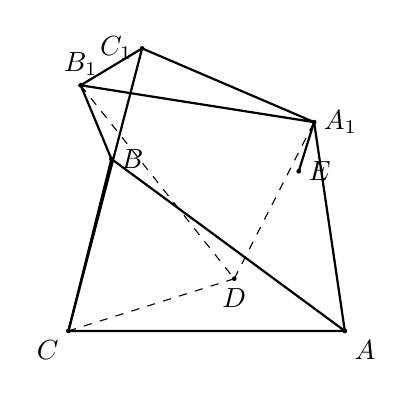
\begin{tikzpicture}[scale=0.78,>=stealth]
  \coordinate (A) at (4.5,0);
  \coordinate (C) at (0,0);
  \coordinate (B) at (0.7,2.8);
  \coordinate (A1) at (4.0,3.4);
  \coordinate (C1) at (1.2,4.6);
  \coordinate (B1) at (0.2,4.0);
  \coordinate (D) at (2.7,0.85);
  \coordinate (E) at (3.75,2.6);
  \draw[thick] (A)--(B)--(C)--(A);
  \draw[thick] (A1)--(B1)--(C1)--(A1);
  \draw[thick] (A)--(A1) (B)--(B1) (C)--(C1);
  \draw[dashed] (B1)--(D) (D)--(A1) (D)--(C);
  \draw[thick] (E)--(A1);
  \fill (A) circle (1.1pt) node[below right] {$A$};
  \fill (B) circle (1.1pt) node[right] {$B$};
  \fill (C) circle (1.1pt) node[below left] {$C$};
  \fill (A1) circle (1.1pt) node[right] {$A_1$};
  \fill (B1) circle (1.1pt) node[above] {$B_1$};
  \fill (C1) circle (1.1pt) node[left] {$C_1$};
  \fill (D) circle (1.1pt) node[below] {$D$};
  \fill (E) circle (1.1pt) node[right] {$E$};
\end{tikzpicture}
\end{center}
\nopagebreak[4]
（1） 求证：$BC\perp A_1B,\ BC\perp A_1A,\ A_1A\perp A_1B$。

（2） 求异面直线 $A_1A$ 和 $BC$ 的距离。

\end{question}
\begin{question}
\gkti{4}

\Needspace{5\baselineskip}
第二卷第三题（本题满分 13 分）。已知复数

\nopagebreak[4]
\[
z=\cos\alpha+i\sin\alpha,\qquad
u=\cos\beta+i\sin\beta,
\]

\Needspace{5\baselineskip}
且

\nopagebreak[4]
\[
z+u=\frac45+\frac35i.
\]

（1） 求 $\operatorname{tg}(\alpha+\beta)$ 的值；

\Needspace{5\baselineskip}
（2） 求证：

\nopagebreak[4]
\[
z^2+u^2+zu=0.
\]

\end{question}
\begin{question}
\gkti{5}

\Needspace{5\baselineskip}
第二卷第四题（本题满分 15 分）。直线 $l$ 过抛物线

\nopagebreak[4]
\[
y^2=2px\qquad(p\ne0)
\]

的焦点，并且与这抛物线相交于 $A(x_1,y_1)$ 和 $B(x_2,y_2)$ 两点。

\Needspace{5\baselineskip}
（1） 求证：

\nopagebreak[4]
\[
4x_1x_2=p^2.
\]

（2） 求证：对于这抛物线的任何给定的一条弦 $CD$，直线 $l$ 不是 $CD$ 的垂直平分线。

\end{question}
\begin{question}
\gkti{6}

\Needspace{5\baselineskip}
第二卷第五题（本题满分 15 分）。设实数 $a\ne0$，数列 $\{a_n\}$ 是首项为 $a$、公比为 $-a$ 的等比数列，记

\nopagebreak[4]
\[
b_n=a_n\lg|a_n|,\qquad n=1,2,\ldots,
\]

\nopagebreak[4]
\[
S_n=b_1+b_2+\cdots+b_n,\qquad n=1,2,\ldots.
\]

\Needspace{5\baselineskip}
（1） 求证：当 $a\ne-1$ 时，对任意自然数 $n$，都有

\nopagebreak[4]
\[
S_n=\frac{a\lg|a|}{(1+a)^2}
\left[1+(-1)^{n+1}(1+n+na)a^n\right].
\]

（2） 当 $0<a<1$ 时，是否存在自然数 $M$，使得对任意自然数 $n$，都有 $b_n\leq b_M$？证明你的结论。

\end{question}